\documentclass[10pt, letterpaper]{report}
% !TeX program = xelatex
%==================PREAMBOLO=======================%
\input{../../preamble/preamble.tex}
\newcommand{\titolo}{Medical Robotics }

 %TOGLI COMMENTO SE USI XELATEX
%\usepackage{fontspec}
\title{\titolo} %========TITOLO========%
\author{Marco Casu}
\date{\vspace{-5ex}}
\begin{document}

%==================COPERTINA=======================%
\begin{titlepage}
    
\begin{center}
    %TOGLI COMMENTO SE USI XELATEX
   %\setmainfont{Palace Script MT}
   \HUGE Marco Casu\acc
\end{center}
\thispagestyle{empty}
\begin{figure}[h]
    \centering{
        %l'immagine deve avere una risoluzione 2048x2048
        \includegraphics[width=0.95\textwidth ]{images/Copertina.png}
    }
\end{figure}
\vfill 
\centering \includegraphics[width=0.4\textwidth ]{../../preamble/Stemma_sapienza.png} \acc
\centering \Large \color{sapienza}Faculty of Information Engineering, Computer Science and Statistics\\
Department of Computer, Control and Management Engineering\\
Master's degree in Artificial Intelligence and Robotics
\end{titlepage}

%===================FINE COPERTINA======================%
\newpage
%\pagecolor{cartaRiciclata}%\setmainfont{Algerian}
\Large
This document summarizes and presents the topics for the \titolo course for the Master's degree in Artificial Intelligence and Robotics at Sapienza University of Rome. The document is free for any use. If the reader notices any typos, they are kindly requested to report them to the author.
\vfill
\begin{figure}[h!]
    \raggedright
    \includegraphics[width=0.4\textwidth,right ]{../../preamble/tomodachi.pdf} 
\end{figure}
\newpage %\setmainfont{Times New Roman}
\normalsize

\tableofcontents 
\newpage

%==================FOOTER e HEADER=======================%
\fancyhf{}
\fancyhead[L]{\nouppercase{\leftmark}}
\fancyhead[R]{Section \thesection}
\fancyfoot[C]{\thepage}
\fancyfoot[L]{\titolo}
\fancyfoot[R]{ Marco Casu}
%\fancyfoot[R]{\setmainfont{Palace Script MT}\huge Marco Casu \setmainfont{Times New Roman}}
%==================FOOTER e HEADER=======================%
\newtheorem{definition}{Definition}
\newtheorem{proposition}{Proposition}
\newtheorem{theorem}{Theorem}
%==================INIZIO======================%
\chapter{Introduction}
Robotics have entered the domain of healthcare in the last three decades, nowadays we have tools for clinicians and surgeons, robots and mechatronic tools for therapy and training. We distinguish mechatronic tools from the robots, the latter includes some ''autonomous behavior''. The field of medical robotics have evolved to deals with different types of materials, from rigid to soft (usually harder to model), and to operate from the macro to the micro size. Some kinds of surgical operation requires an open access to the body, others ar \textit{minimally invasive}, a classic configuration is the following
\begin{center}
    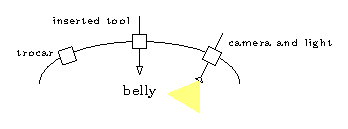
\includegraphics[width=0.7\textwidth]{images/min_invasive_surg.eps} 
\end{center}
where the \textit{trocar} are cylinder-shaped devices used to create small holes in the body to let the surgical tools held by the robots enter (usually equipped with lights and cameras).

Usually, medical robots require an high cost of installation and maintenance, and an increased size of cognitive load for surgeons and staff to operates with these devices, situation awareness is critical. Medical devices also have to pass through a long process of certification.

Differently from the industrial domain, the medical robotics have to take in account one additional variable, the \textit{human being}, that has to be considered in the control loop, both the patient and the surgeon that tele operates the robot.\bigskip
\subsection{Surgical Function and Robot Specifications}
Is important to be able to match a specific surgical function to the relative needed robot, different domains of surgical operation requires different robotic tasks, kinematic structures, control modality, sensors and actuators.
\subsection{Orthopedics}
In the domain of orthopedics, is required the \textit{machining of rigid surfaces}, like cutting, milling and drilling.
\begin{center}
    \includegraphics[width=0.9\textwidth]{images/knee_replacement.png} 
\end{center}
In this context the accuracy that comes from the use of a robot is crucial, since these kind of operations are critical due to the risk of \textit{misplacement of the mechanical axis}, leading to  further loosening of the prosthesis. The use of a robotic agent can help in different situations, for example, an operation can be planned on a simulated environment, and then transferred with a probe that, by touching the knee in different parts, reconstruct the trajectories to be performed and localize the coordinates.

The main advantages of this operation is the accuracy, permitting a smaller footprint in the patient, since robot are more accurate, with a smaller workspace, leading to intrinsically safer operations.

A completely different approach are the \textit{bone mounted robot}, where a structure is mounted on the patient, in such way even if the subject moves, the alignment of the tools is preserved, in this way we get minimal obstruction, patient immobilization and a small workspace. These approach are specific to spine surgery and the integration in the surgery workflow not smooth.
\end{document}